\documentclass[12pt,a4paper]{article}

\usepackage[T1]{fontenc}
\usepackage[utf8]{inputenc}
\usepackage[english]{babel}
\usepackage{amsmath,amssymb}
\usepackage{graphicx}
\usepackage{geometry}
\usepackage{hyperref}
\geometry{margin=2.5cm}
\graphicspath{{figures/}}
\hypersetup{colorlinks=true,linkcolor=blue,urlcolor=blue}

\title{\textbf{Implementing a PINN with\\ NumPy and Numba (CUDA)}}
\author{Nikita Sviridov}
\date{\small(translated from the Russian original)}

\begin{document}
\maketitle

\section{Introduction}

A PINN (Physics-Informed Neural Network) is a network designed to solve
differential equations. The task can be viewed as unsupervised learning, because
no labels are needed to train the network. The loss is computed from the
differential equation itself, together with the boundary and initial conditions.

The network is trained so that, when the function it represents is substituted
into our PDE, BCs and ICs, the deviations from the true values are minimal.

\section{The differential equation}

I chose the heat equation --- a partial differential equation of up to second
order:
\begin{equation*}
\begin{cases}
\dfrac{\partial u}{\partial t} = \Delta u + x\,t^2 \sin y, & 0 < x < 1,\ 0 < y < \tfrac{\pi}{2},\ t > 0,\\[2mm]
\dfrac{\partial u}{\partial x}\Big|_{x=0} = \dfrac{\partial u}{\partial x}\Big|_{x=1} = 0, & \\[2mm]
u\big|_{y=0} = 0, \quad \dfrac{\partial u}{\partial y}\Big|_{y=\pi/2} = 0, & \\[2mm]
u\big|_{t=0} = 0. &
\end{cases}
\end{equation*}

\section{Network architecture}

The architecture is a 4-layer multilayer perceptron with a sigmoid activation
between layers:
\[
\sigma\!\big(\sigma(\sigma(X A_1 + B_1)A_2 + B_2)A_3 + B_3\big)A_4 + B_4,
\]
where $A_i$ is the weight matrix of a layer and $B_i$ its bias (added row-wise),
and
\[
\sigma(x) = \frac{1}{1 + e^{-x}}
\]
is the sigmoid activation. Weights are initialized with the Xavier method:
matrix entries are drawn from a normal distribution
$\mathcal{N}\!\big(0, 1/\dim_{\text{in}}\big)$.

\section{Implementation}

There are two stages. The first is writing the training algorithm itself; the
second is moving the computation onto CUDA.

\subsection{The algorithm}

A neural network can be seen as a large parameterized function. Training its
parameters, like any model, is based on gradient descent: a loss function is
defined, an error is computed from it during training, and then the parameter
gradients are obtained. Since the gradient points in the direction of increase,
the parameters are shifted along the negative gradient to minimize the error.

Rather than deriving per-layer gradient formulas by hand, I wrote a general form
of the network and trained that. By ``general form'' I mean an
automatic-differentiation system --- a wrapper class (\texttt{tensor}) over an
ordinary tensor that records the gradient of every arithmetic operation at each
step. This makes it possible to compute the gradient of any node in the
computation graph by backpropagation. Because the backward functions are
themselves expressed as tensor operations, the gradient graph is also
differentiable --- which is exactly what allows taking the second-order
derivatives ($u_{xx}$, $u_{yy}$) required by the equation.

\subsection{Parallel computation}

To make the network run in reasonable time, the computation is moved onto CUDA.
This requires solving the data-allocation problem: training is a dynamic process
in which hundreds of constructors and destructors of our class are called at each
step. Moving matrices to the GPU during training is inefficient, so a large block
of memory is allocated up front and we operate within it.

I wrote a wrapper over the allocated memory, \texttt{memory\_manager}, to which
allocation and reclamation are delegated. When a new tensor is needed, a free
region is selected and marked as used; when the destructor is called, the region
becomes available again. Region selection uses a greedy fragmentation-minimizing
strategy: free intervals are kept sorted by size and the best fit is found in
logarithmic time via binary search. On free, the region is merged with adjacent
free intervals.

The parallelized functions fall into three categories:
\begin{itemize}
  \item arithmetic operations;
  \item memory filling;
  \item reduce operations.
\end{itemize}

\emph{Arithmetic operations.} Implemented: matrix multiplication; elementwise
addition, multiplication, division and exponentiation; elementwise $\ln$,
$\cos$, $\sin$. The matrix multiply uses a tiled (block) algorithm with shared
memory. All binary operators are also defined for the case where the second
argument is a scalar.

\emph{Memory filling.} Implemented: filling a matrix with another matrix or a
scalar, taking a slice of a matrix, and writing into a slice.

\emph{Reduce operations.} Implemented: summation of all elements, summation
along columns, and summation along rows.

All computation is implemented in two interchangeable backends: pure NumPy (CPU)
and CUDA kernels (Numba). The autodifferentiation graph is identical for both.

\section{Training}

\emph{Loss function.} The loss is a sum of three kinds of terms: the first
enforces the differential equation, the second the boundary conditions, and the
third the initial condition:
\[
\text{Loss} = \Big\| \tfrac{\partial u_{\text{pinn}}}{\partial t} - \Delta u_{\text{pinn}} - x t^2 \sin y \Big\|
 + \sum_{i=1}^{4} \big\| \mathrm{BC}_i(u_{\text{pinn}}) \big\|
 + \big\| \mathrm{Init}(u_{\text{pinn}}) \big\|,
\]
where $\mathrm{BC}_i$ is the boundary-condition operator and $\mathrm{Init}$ the
initial-condition operator.

\emph{Training parameters.} Plain gradient subtraction is not optimal, so a more
advanced method --- Adam --- is used. My implementation is canonical Adam with
bias correction of the moments ($\hat{m}$, $\hat{v}$). A learning rate of $0.01$
worked best; the number of epochs was set to $2000$ as a trade-off between
training time and accuracy.

\emph{Batch sizes in the loss terms.} At each epoch, points are sampled at random
from the domain over which the solution is sought. For the PDE error, points are
taken from the 3-D space $(x, y, t)$; for the ICs and BCs one coordinate is
fixed. The PDE error is averaged over $200$ points, and each BC/IC error over
$50$ points.

\section{Comparison with the analytic solution}

The analytic solution is obtained by separation of variables and expanding the
source in a Fourier series in cosines (which satisfy the Neumann conditions in
$x$) and in $\sin y$ (which satisfies the conditions in $y$). The maximum
absolute deviation of the numerical solution from the analytic one does not
exceed $\approx 0.01$ at $t = 1$.

\begin{figure}[h]
\centering
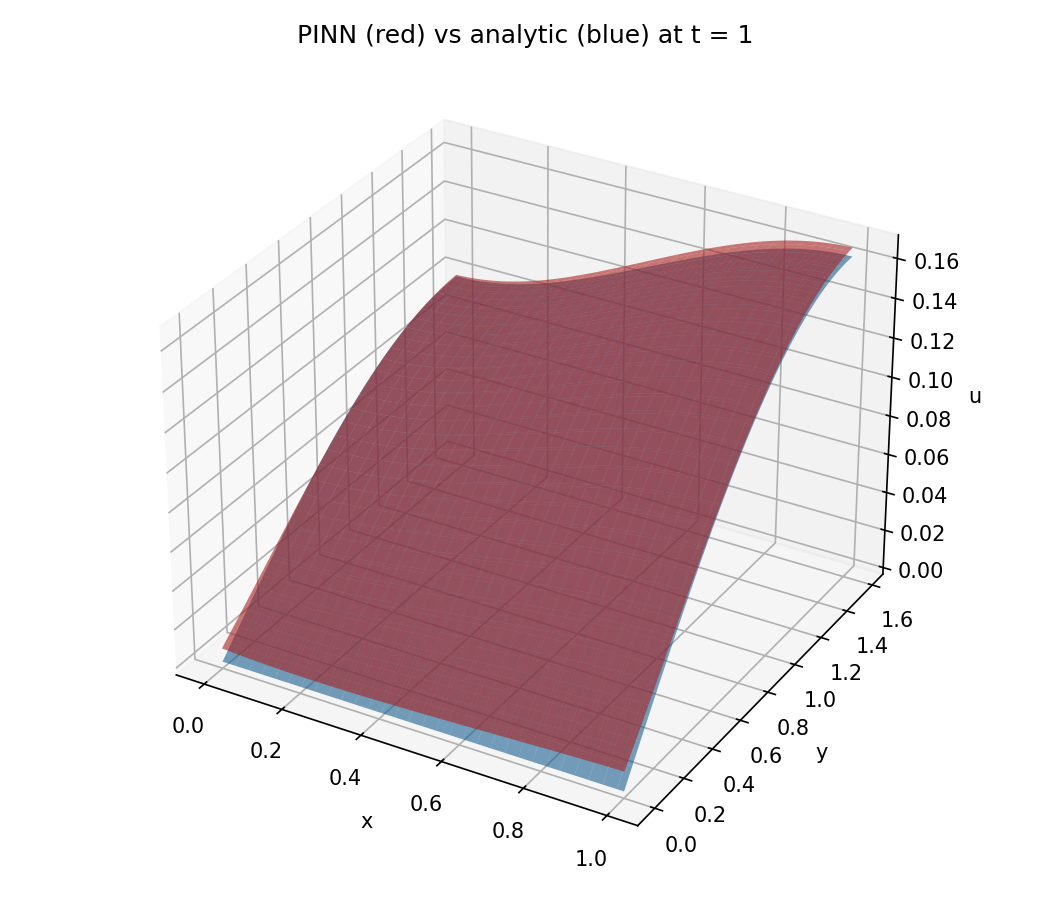
\includegraphics[width=0.48\textwidth]{comparison_t1.png}
\hfill
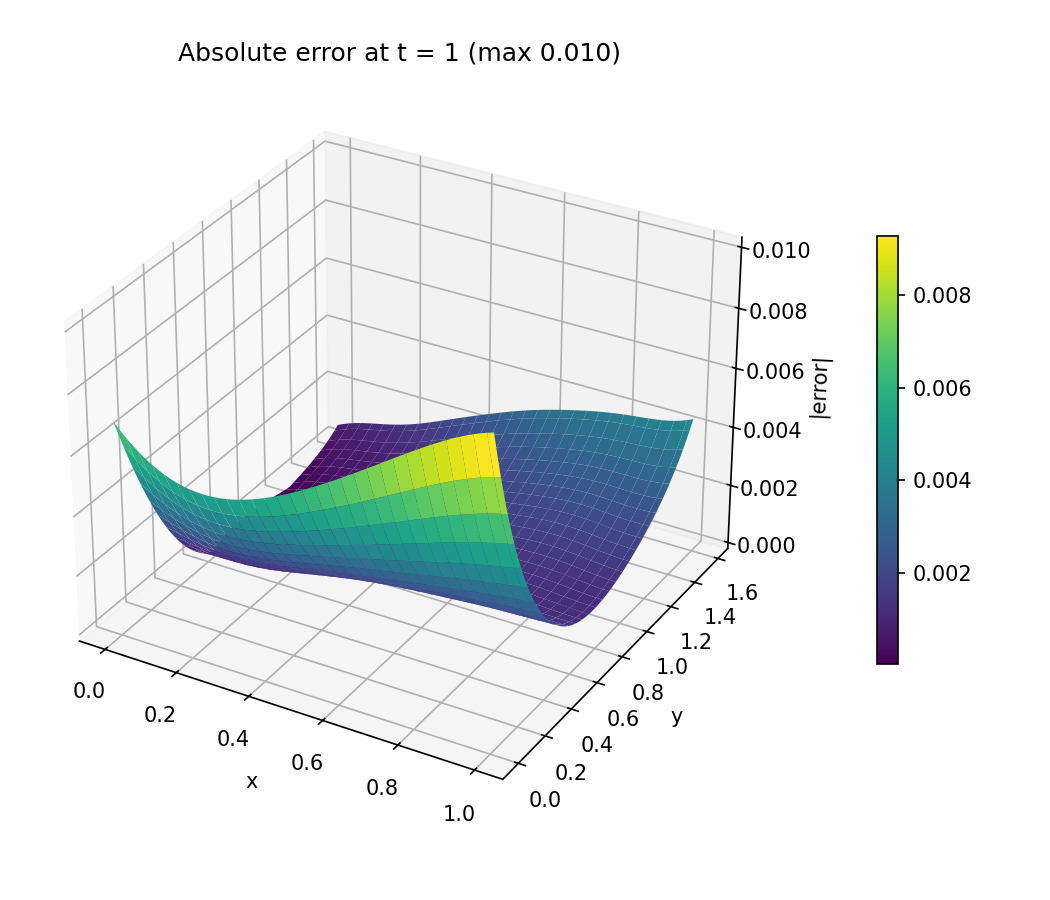
\includegraphics[width=0.48\textwidth]{error_field.png}
\caption{Left: comparison with the analytic solution (blue --- analytic,
red --- numerical). Right: absolute-error field at $t = 1$.}
\end{figure}

\begin{figure}[h]
\centering
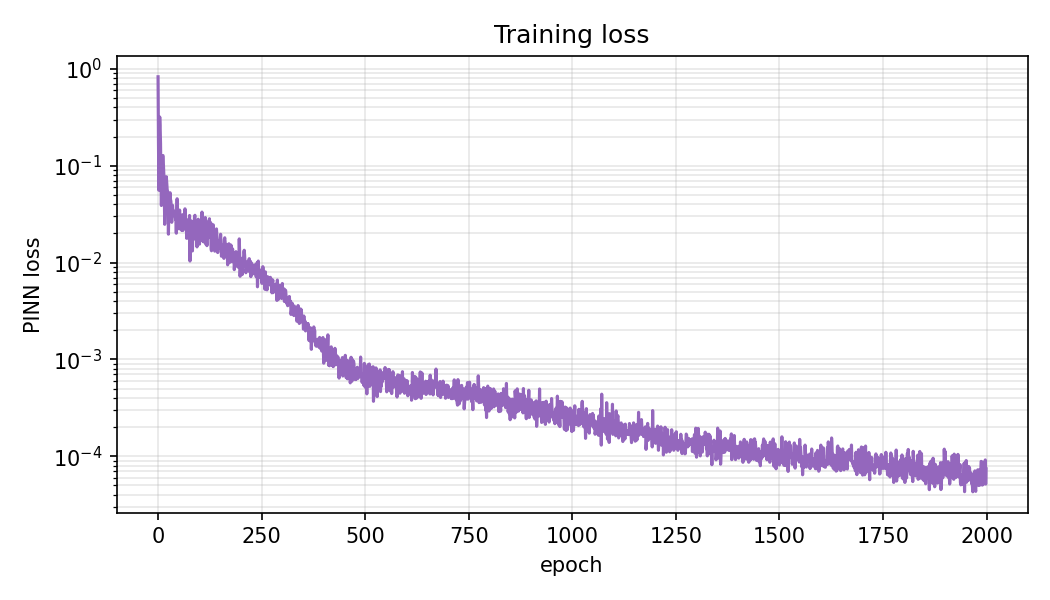
\includegraphics[width=0.7\textwidth]{loss_curve.png}
\caption{Training loss over epochs (logarithmic scale).}
\end{figure}

On the relevance of solving PDEs with PINNs: the approach can compete with other
numerical PDE solvers --- with library implementations the number of epochs can
be increased substantially and the accuracy improved by orders of magnitude.

\section{Performance}

I compared automatic differentiation running on CUDA versus plain NumPy. At the
small matrix sizes used in this architecture (no axis exceeds a few hundred), the
GPU is under-utilized, so the dominant cost is not the computation itself but the
orchestration: thousands of tiny kernel launches per epoch and an
autodifferentiation graph built from Python objects. This also explains why the
from-scratch implementation is slower than PyTorch: its dispatch and graph are
implemented in C++ and its operations are fused. The bottleneck, therefore, is
not the kernel language but the orchestration and the problem size.

\end{document}
